\newpage

\chapter{\textsc{огляд технології FHE}}


\section{Визначення}
В цій секції описана термінологія, яка використовується в дослідженнях FHE. Деякі з 
визначень були взяті напряму з документів FHE, інші були перефразовані для того, щоб
спростити формальність і зробити їх більш застосованими до обраної задачі.

Нехай є простір вхідного (чистого) тексту \(\mathcal{P}=\{0,1\}\), та сімейства функцій
\(F={f_1,f_2,...,f_n}\) де \(f_n(x) = f(x_1,x_2,x_3,...,x_k)\) це Булеві функції k
аргументів: \(f: P^n \rightarrow P\). Ми будемо називати F, сімейством Булевих схем
(Boolean circuit) \(C\), і використовувати звичайний запис функції \(C(m_1,m_2,...,m_n)\),
для позначення оцінки Булевої схеми на кортежі \((m_1,m_2,...,m_n)\).

\begin{definition}[\(\mathcal{C}\)-схема розрахунків, або ж просто \(\mathcal{C}\)-схема \cite{cryptoeprint:2011/344}] 
    Нехай \(\mathcal{C}\) це множина Булевих схем, тоді \(\mathcal{C}\)-схема розрахунків, для
    \(\mathcal{C}\) це набір функцій \((\textsc{gen, enc, eval, dec})\) які задовільняють наступним твердженням:


\(\textsc{\textbf{gen}}(1^\lambda,\alpha)\) - алгоритм генерації ключів, на вхід він приймає,
параметр шифрування \(\lambda\), та допоміжний параметр \(\alpha\). Результат виконання
алгоритму це триплет ключів \((pk,sk,evk)\), де ключ \(pk\) використовується для шифрування,
\(sk\) для дешифрування, та  \(evk\) для виконування розрахунків.

\(\textsc{\textbf{enc}}(pk,m)\) - алгоритм шифрування, на вхід він приймає ключ шифрування \(pk\) та
фрагмент не зашифрованого (чистого) тексту \(m\). Результат виконання алгоритму це шифр \(c\).

\(\textsc{\textbf{eval}}(evk,C,c_1,c_2...,c_n)\) - алгоритм розрахунків. На вхід він отримує,
ключ розрахунків \(evl\) та Булеву схему \(C \in \mathcal{C}\), та вхідні аргументи, які
можуть бути як шифром, так і результатом виконання минулих розрахунків. Результат виконання
алгоритму це результат виконання розрахунків.

\(\textsc{\textbf{dec}}(sk, c)\) - алгоритм дешифрування. На вхід приймає, ключ дешифрування
\(sk\), та шифр, або результат виконання розрахунків. Результат виконання алгоритму це не
зашифрований (чистий) текст \(m\).
\end{definition}

Для подальшого опису властивостей, треба визначити простори даних, які є результатами, або
вхідними параметрами описаних алгоритмів:

Нехай \(\mathcal{X}\) буде описувати простір \emph{чистого шифру}, \(\mathcal{Y}\) -
простір результатів виконання розрахунків, і \(\mathcal{Z} = \mathcal{X} \cup \mathcal{Y}\).
\(\mathcal{Z^*}\) - містить кортежі довільної довжини, які складаються
з елементів \(\mathcal{Z}\). Простори ключів згенерованих \textsc{\textbf{gen}},
позначимо як \(\mathcal{K}_p,\mathcal{K}_s,\mathcal{K}_e\) для \(pk,sk,evk\) відповідно.Алгоритм \textsc{\textbf{gen}} приймає на вхід параметр в унарній нотації \(1^\lambda\)
та опціональний допоміжний параметр \(\lambda\) з простору \(\mathcal{A}\). Також,
\(\mathcal{C}\) містить простір \emph{дозволених} булевих схем, а \(\mathcal{P}\), як було
зазначено раніше, область вхідного \emph{чистого (незашифрованого)тексту}.

Тепер можна описати область роботи наведених вище алгоритмів:
\begin{center}
    \begin{tabular}{l}
        \textsc{\textbf{gen }}: 
        \begin{math}
            \mathbb{N}\ \times\ \mathcal{A}\ \rightarrow\ 
            \mathcal{K}_p\ \times\ \mathcal{K}_s\ \times \ \mathcal{K}_e
        \end{math}\\

        \textsc{\textbf{enc }}:
        \begin{math}
            \mathcal{K}_p\ \times\ \mathcal{P}\ \rightarrow\ \mathcal{X}
        \end{math}\\

        \textsc{\textbf{eval}}:
        \begin{math}
            \mathcal{K}_e\ \times\ \mathcal{C}\ \times\ \mathcal{Z}^*\ 
            \rightarrow\ \mathcal{Y}
        \end{math}\\

        \textsc{\textbf{dec }}:
        \begin{math}
            \mathcal{K}_s\ \times\ \mathcal{Z}\ \rightarrow\ \mathcal{P}
        \end{math}
    \end{tabular}
\end{center}

Тоді \(\mathcal{X}\) та \(\mathcal{Y}\) можна визначити наступним чином:
\begin{center}
    \begin{math}
        \mathcal{X}\ =\ \{c\ |\ \textsc{\textbf{enc}}(pk,m)\ =\ c,\ m\ \in\ \mathcal{P}\}
    \end{math}
    \begin{math}
        \mathcal{Y}\ =\ \{z\ |\ \textsc{\textbf{eval}}(evk,C,c_1,c_2,...,c_n) = z,\ c_i\ \in\ 
        \mathcal{Z},\ C\ \in\ \mathcal{C} \}
    \end{math}
\end{center}
В деяких схемах, ключі розрахунків та шифрування однакові, але часто це і не так, тому в
визначеннях було наведено більш спільний випадок.

В оригінальних документах FHE \cite{cryptoeprint:2011/344} не було зазначено, що алгоритм
розшифровування \textsc{\textbf{dec}} повинен мати можливість працювати з результатом виконання
алгоритму шифрування \textsc{\textbf{enc}} - \(\mathcal{X}\), і було зазначено, що данні
можуть бути розшифровані після виконання розрахунків над ними \textsc{\textbf{eval}} - 
\(\mathcal{Y}\). Для можливості розшифровування, зразу після зашифровування було запропоновано
мати \emph{чисту Булеву схему} або ж по суті функцію \(f(x)=x\), для виконання розрахунків і
отримання даних які вже можна буде розшифровувати. Більшість сучасних FHE схем, дозволяють
проводити операції дешифрування даних, над якими не було проведено розрахунків, тому я не буду
заглиблюватись в цю тему.

\subsection{Атрибути та властивості}
Тут представлені характеристики методів гомоморфного шифрування. Ми встановлюємо такі
властивості, як компактність і конфіденційність схеми, які забороняють спрощені рішення
задачі гомоморфного шифрування, з одного боку, і вимагають таких властивостей, як
коректність, для того, щоб навіть називати це схемою шифрування.

\begin{definition}[Коректне розшифровування \cite{cryptoeprint:2015/1192}]
\label{def:corr-dec}
\(\mathcal{C}\)-схама має атрибут коректного розшифрування якщо виконується наступне твердження:
\begin{center}    
    \begin{math}
        \textsc{\textbf{dec}}(sk,\textsc{\textbf{enc}}(pk,m)) = m
    \end{math},\\
    де \(pk,sk,evk \leftarrow \textsc{\textbf{gen}}(1^\lambda,\alpha)\), \(\alpha \in \mathcal{A}\), \(m \in \mathcal{P}\).
\end{center}
Це означає, що ми повинні мати можливість безпомилково розшифровувати зашифрований текст.
\end{definition}

\begin{definition}[Коректні розрахунки \cite{cryptoeprint:2015/1192}]
\label{def:corr-eval}
\(\mathcal{C}\)-схема коректно розраховує всі Булеві схеми \(C \in \mathcal{C}\), якщо
виконується наступне твердження:
    \begin{center}
        \begin{math}
        \textsc{\textbf{dec}}(sk,\textsc{\textbf{eval}}(evk,C,c_1,c_2,...,c_n))\ 
        =\ C(m_1,m_2,...m_n)
        \end{math},\\
        \(pk,sk,evk \leftarrow \textsc{\textbf{gen}}(1^\lambda,\alpha)\), \(\alpha \in \mathcal{A}\), \(c_i \in \mathcal{X}\) та \(m_i \leftarrow \textsc{\textbf{dec}}(sk,c_i)\)
    \end{center}
Це визначення означає, що розрахунки над зашифрованими даними з подальшим
розшифровуванням повинні бути однакові з результатом розрахунків над не зашифрованими
даними.
\end{definition}

Будемо називати \(\mathcal{C}\)-схему \emph{коректною} якщо для неї будуть виконуватись
\ref{def:corr-dec} та \ref{def:corr-eval} твердження.

\begin{definition}[Компактність \(\mathcal{C}\)-схеми]
\label{def:compactness}
    \(\mathcal{C}\)-схема вважається компактною якщо існує поліном \(p\), такий що, для
    будь-якого кортежу \((pk,sk,evk) \leftarrow \textsc{\textbf{gen}}(1^\lambda,\alpha)\), \(\alpha \in \mathcal{A}\), будь-якої Булевої схеми \(C \in \mathcal{C}\) та
    шифру \(c_i \in \mathcal{X}\), розмір результату виконання
    \(\textsc{\textbf{eval}}(evk,C,c_1,c_2,...,c_n)\) не більше від \(p(\lambda)\)
    бітів, в не залежності від Булевої схеми.
\end{definition}
Визначення \ref{def:compactness}, показує що під час гомоморфних операцій розмір
результату не повинен збільшуватись, і залежить тільки від параметра безпеки \(\lambda\).

\begin{definition}[Компактно розрахункова \(\mathcal{C}\)-схема \cite{homenc}]
\label{def:compactl-eval}
\(\mathcal{C}\)-схема компактно розраховує всі Булеві схема \(C \in \mathcal{C}\), якщо
вона компактна \ref{def:compactness} та \emph{коректна}.
\end{definition}

\subsubsection*{Безпека схеми}
Далі, важливо зупинитись на безпеці та конфіденційності схеми. Безпеку схеми можна
розділити на дві компоненти: семантична безпека, та обфускація схеми. Якщо обфускація
використовується коли алгоритм шифрування секретний, і вразливий, то семантична безпека
описує розподіл вихідних даних з \textsc{\textbf{eval}} та \textsc{\textbf{enc}}.
\begin{definition}[Приватне гомоморфне шифрування схеми \cite{homenc}(2.16)]
    \(\mathcal{C}\)-схема вважається безпечною, якщо для будь-якого кортежу \((pk,sk,evk) \leftarrow \textsc{\textbf{gen}}(1^\lambda,\alpha)\), \(\alpha \in \mathcal{A}\), будь-якої Булевої схеми \(C \in \mathcal{C}\) та
    шифру \(c_i \in \mathcal{X}\), такого що \(m_i \leftarrow \textsc{\textbf{dec}}(sk, c_i)\) існує два розподіли:

\begin{center}
    \begin{math}
        Dist_1 = \textsc{\textbf{eval}}(evk,C,c_1,c_2,...,c_n)
    \end{math}\\
    \begin{math}
        Dist_2 = \textsc{\textbf{enc}}(pk,C(c_1,c_2,...,c_n)
    \end{math}
\end{center}
які повинні бути статистично або обчислювально нерозрізнені. Ці вимоги показують,
що розподіл виконання обчислень Булевої схеми над шифром \(Dist_1\) повинен бути однаковий (статистично, обчислювально) з розподілом, отриманим шляхом зашифровування
\emph{чистого} тексту, який насамперед являється результатом виконання Булевої операції 
над незашифрованими даними \(Dist_2\).

Часто термін безпечної системи можна зустріти як \emph{Сильно гомоморфна система}\cite{Clear_2013}. 
\end{definition}

\subsection{Класифікація}
Оскільки не всі схеми FHE мають однакові властивості, цей розділ показує як схеми
класифікуються, в залежності від того, які схеми вони можуть обчислювати.

\begin{definition}[Частково Гомоморфна схема або \(\mathcal{C}\)-Гомоморфізм \cite{cryptoeprint:2011/344}]
\(\mathcal{C}\)-схема називається, частково гомоморфною (SHE), якщо вона має коректне
шифрування \ref{def:corr-dec}, та коректне обчислення \ref{def:corr-eval}.
\end{definition}
Для частково гомоморфних \(\mathcal{C}\)-схем нема вимог до компактності, тому з кожним
гомоморфним розрахунком розмір вихідного шифру може збільшуватись. Також нема ніяких
вимог до множини Булевих операцій які можуть бути використовувані для розрахунків.

\begin{figure}[!ht]
    \centering
    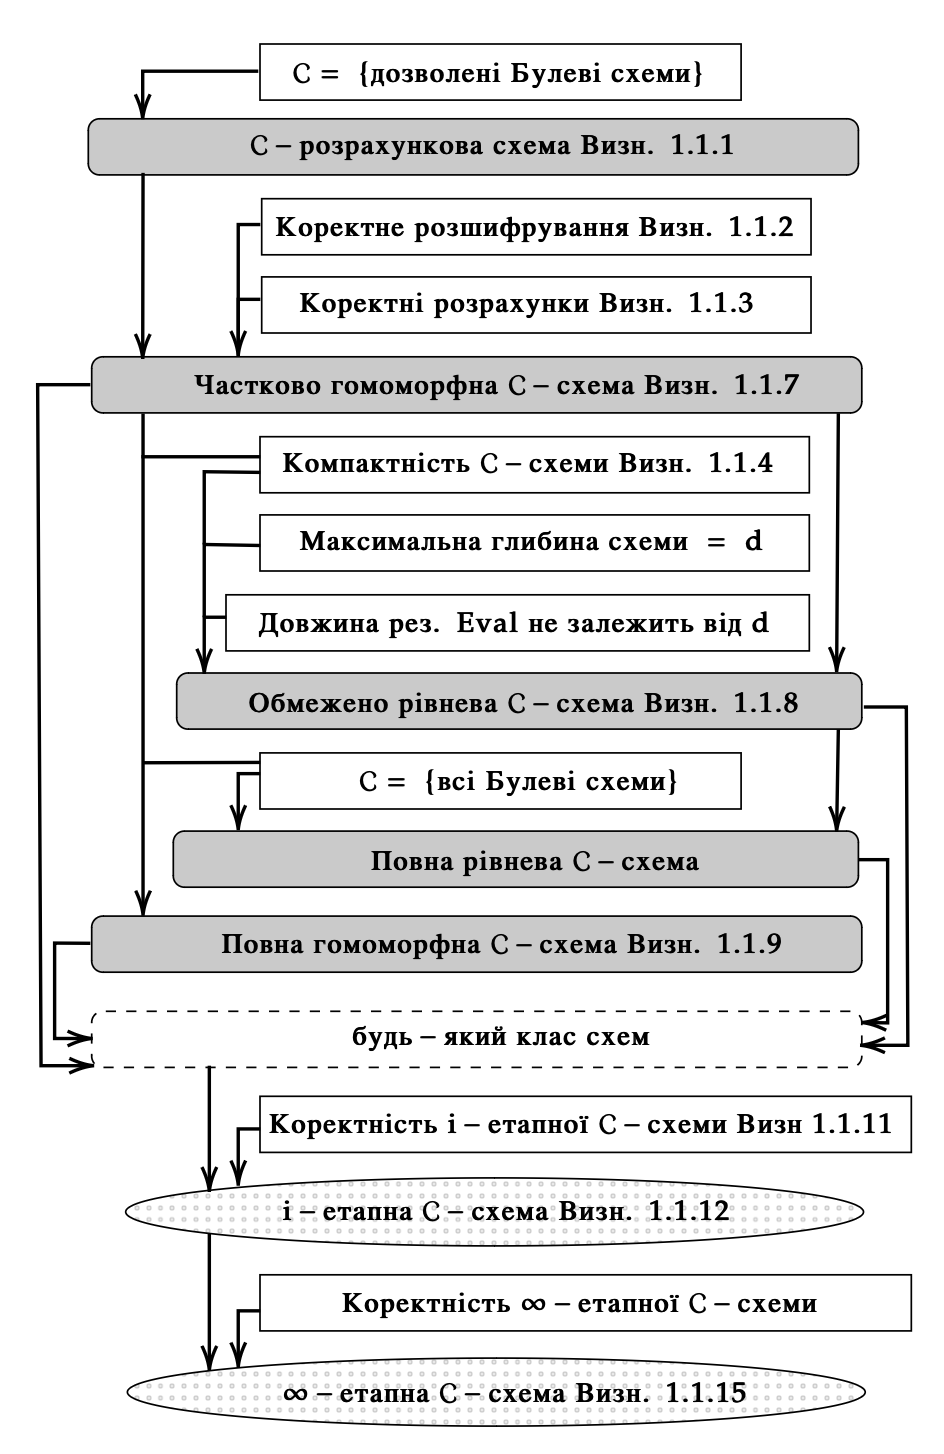
\includegraphics[scale=0.75]{static/classification.png}
    \caption{Дерево класифікацій \(\mathcal{C}\)-схем. Прямокутниками позначені визначення,
    закруглені затемнені прямокутники, позначають класи \(\mathcal{C}\)-схеми, а еліпси
    позначають розширення для етапних розрахунків. Стрілки показуть залежність одного 
    твердження від іншого.}
    \label{fig:classification}
\end{figure}

\begin{definition}[Обмежено-рівнева Гомоморфна схема]
\(\mathcal{C}\)-схема називається Обмежено-рівневою, якщо алгоритм генерації ключів
\textsc{\textbf{gen}} приймає додатковий параметр \(\alpha=d\), який означає максимальну
глибину Булевої схеми, яка може бути обчислена. Також застосовані вимоги до компактності,
коректності, і те що розмір вихідних даних розрахунків не повинен залежати від d.

\end{definition}

\begin{definition}[Повна Гомоморфна схема]
Повною гомоморфною схемою, називають \(\mathcal{C}\)-схему, до якої застосовані вимоги,
коректності, компактності, та вона може обчислювати Булеву схему з множини усіх схем, або
ж будь-яку схему.
\end{definition}

\subsection{Композиція розрахунків}
Часто, задача потребує декілька послідовних розрахунків, тобто результат певної Булевої
схеми повинен слугувати вхідними даними для наступної схеми, або ж простими словами
можна це назвати - композиція.
Кожну операцію розрахунків над шифром \textsc{\textbf{eval}} будемо називати \emph{етапом розрахунків}. 

З визначення коректних розрахунків \ref{def:corr-eval} видно що вхідні дані для
алгоритму обчислення \textsc{\textbf{eval}} повинні належати множині \(\mathcal{X}\) -
або ж множині \emph{чистого шифру}, який є результатом алгоритму \textsc{\textbf{enc}}.
Цей розділ описує вимоги, виконуючи які алгоритм розрахунку схеми \textsc{\textbf{eval}},
може приймати на вхід як результат виконання інших розрахунків \(\mathcal{Z}\), так і
\emph{чистий шифр} \(\mathcal{X}\): 

\(\textsc{\textbf{eval}}(evk, C, c_1,c_2,...,c_n)\),
де \((pk,sk,evk) \leftarrow \textsc{\textbf{gen}}(1^\lambda,\alpha)\), \(\alpha \in \mathcal{A}\), \(C \in \mathcal{C}\) та \(c_i \in \mathcal{X} \cup \mathcal{Z}\)

В літературі \emph{розрахунки з етапами} називають \textbf{\emph{гомоморфним шифруванням
з i-етапами}}(i-hop homomorphic encryption \cite{10.1007/978-3-642-19571-6_14},
\cite{cryptoeprint:2010/145})

\begin{definition}[Розрахунки з етапами]
\label{def:stage-eval} 
    Обчислення \(\textbf{C}_{i,n}\) в \(i\) етапів, та шириною \(n\), визначається множиною
    Булевих схем \(\{C_{kl}\}\), де \(1 \leq k \leq i,1 \leq l \leq
    \) n, та \(C_{kl}\) має \(kn\) вхідних даних. За вхідними даними \(m_{01},m_{02},...,m_{0n}\) ми
    обчислюємо:
\begin{center}
    \(m_{kl} = C_{kl}(m_{01},m_{02},...,m_{0n},...,m_{k-1,1},...,m_{k-1,n})\), де \(1 \leq k \leq i,1 \leq l \leq n\).
\end{center}
Результат розрахунків з етапом після \textsc{\textbf{eval}} та \textsc{\textbf{dec}} буде 
\emph{чистий текст} \(m_{i1},m_{i2},...,m_{in}\). Визначимо початковий \emph{чистий текст} як
\(\overrightarrow{m_0}\), та вихідний \emph{чистий текст} як \(\overrightarrow{m_i}\), тоді можна
записати співвідношення \(\overrightarrow{m_i} = C_{i,n}(\overrightarrow{m_0})\).


Нехай \((pk,sk,evk) \leftarrow \textsc{\textbf{gen}}(1^\lambda,\alpha)\), \(\alpha \in \mathcal{A}\),
та \(c_{i1},c_{i2},...,c_{in} \in \mathcal{X}\), тоді шифр \(\{c_{kl}\}\), 
\(1 \leq k \leq i,1 \leq l \leq n\) обчислюється рекурсивно наступним чином:
\begin{center}
    \(c_{kl} = \textsc{\textbf{eval}}(evk,C_{kl},c_{01},...,c_{0n},...,c_{k-1,1},...,c_{k-1,n})\)
\end{center}
Результат розрахунків з етапом над зашифрованими даними, буде шифр \(c_{i1},c_{i2},...,c_{in}\).
Позначивши початковий (вхідний) шифр як \(\overrightarrow{c_0}\) та результівний шифр як 
\(\overrightarrow{c_i}\) можна описати співвідношення яке описує нотацію алгоритму \textsc{\textbf{eval}}
з декількома виходами: \(\overrightarrow{c_i} = \textsc{\textbf{eval}}(evk,C_{1,n},\overrightarrow{c_0})\)
\end{definition}

\begin{figure}[ht!]
    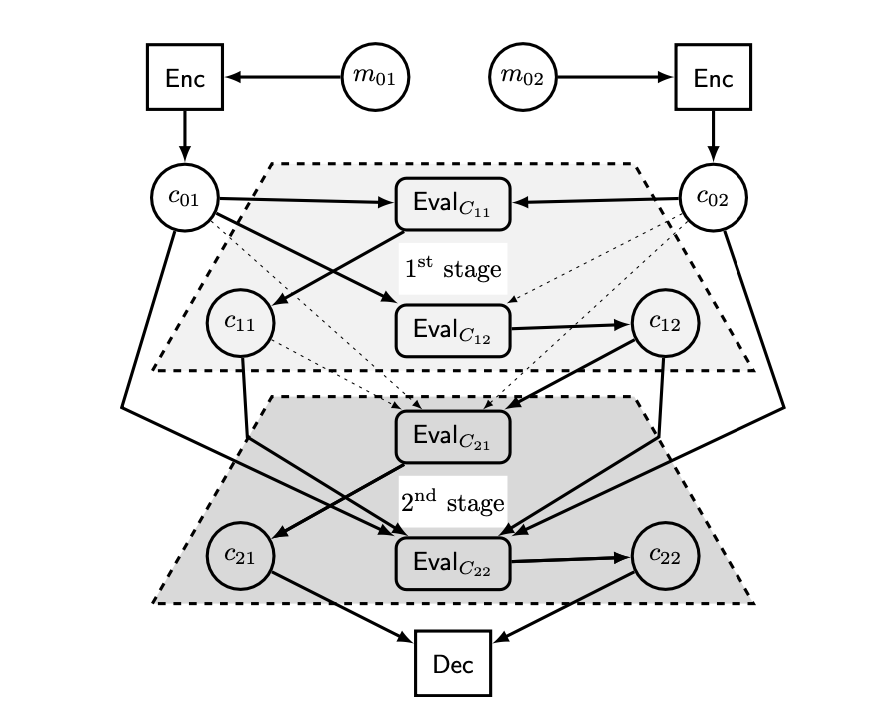
\includegraphics[]{static/I-hop-eval.png}
    \caption{Приклад \cite{cryptoeprint:2015/1192} гомоморфного шифрування з i-етапами,
    де \(i=2,n=2\)}
    \label{fig:i-hop-eval}
\end{figure}

З вище описаного визначення \ref{def:stage-eval} можна зробити висновок що вхідними даними для
будь-якого етапу, окрім першого, може бути \textsc{тільки} результат попереднього етапу.

На перший погляд, може здатись, що якщо у нас є можливість обчислити довільну Булеву схему, не
використовуючи \(i\)-етапне шифрування, то повинна бути можливість обчислювати багато схем
послідовно. Проте це не так. Нема гарантій того, що результат виконання \textsc{\textbf{eval}},
буде валідний для використання як вхідні дані для наступного \textsc{\textbf{eval}}.
Наведемо приклад \cite{cryptoeprint:2015/1192}: Нехай у нас є схема \(C\) яка приймає на вхід
\(c_1,c_0,...,c_n\), та результатом якої є \(c'_0,c'_1,...,c'_v\), та схема \(C'\), яка приймає
на вхід \(c_0,c_1,...,c_v\) та результат якої \(c'_0,c'_1,...,c'_w\). Тоді існує 2 можливих 
сценарії: 1) Якщо ми візьмемо композицію \(C\) та \(C'\) як схему для розрахунків
\textsc{\textbf{eval}}(evk, \(C \circ C'\), \(c_1,c_2,...,c_n\)) то ці розрахунки будуть
коректними, оскільки виконується одна Булева схема, 2) проте, якщо ми спочатку розрахуємо
\textsc{\textbf{eval}}(evk, \(C\), \(c_1,c_2,...,c_n\)) = \(c'_1,c'_2,...,c'_v\), а потім
\textsc{\textbf{eval}}(evk, \(C'\), \(c'_1,c'_2,...,c'_v\)) то це не спрацює зі звичайною
схемою повного гомоморфного шифрування, оскільки вона не гарантує коректність даних після
розрахунків, для наступних операцій. Тому якщо стоїть задача виконання послідовних, незалежних
обчислень, то варто використовувати схему з i-етапами.

\begin{definition}[Коректність гомоморфного шифрування з i-етапами]
\label{def:i-hop-eval-corr}
Нехай \((pk,sk,evk) \leftarrow \textsc{\textbf{gen}}(1^\lambda,\alpha)\), \(\alpha \in \mathcal{A}\),
та \(\textbf{C}_{i,n}=\{C_{k,l}\}\) - довільне поетапне обчислення, де \(n\) це розмір
полінома від \(\lambda\) та \(\overrightarrow{c_0}=(c_{01},c_{02},...,c_{0n}) \in
\mathcal{X}^n\). Тоді \(\mathcal{C}\)-схему можна вважати коректною з і-етапами, якщо
виконується наступне твердження:
\begin{center}
    \begin{math}
        \textsc{\textbf{dec}}(sk,\textsc{\textbf{eval}}(evk,\textbf{C}_{i,n},
        \overrightarrow{c_0})) = \textbf{C}_{i,n}(\textsc{\textbf{dec}}(sk,\overrightarrow{c_0}))
    \end{math}
\end{center}
\end{definition}
Хоча це визначення і дуже схоже на визначення коректності розрахунків \ref{def:corr-eval},
проте важливо розуміти, що наведене вище визначення застосоване до розрахунків з
багатьма етапами, про що свідчить \(\textbf{C}_{i,n}\) = \(\{C_{k,l}\}\).


На Рис. \ref{fig:i-hop-eval} зображений приклад розрахунків з етапами, де \(i=2,n=2\).

Тепер, маючи загальне визначення коректності гомоморфного шифрування, можна описати більш
часткові випадки шифрування з i-етапами, а саме: i-етапне, мульті-етапне, полі-етапне та
\(\infty\)-етапне.

\begin{definition}[i-етапна \(\mathcal{C}\)-схема \cite{cryptoeprint:2010/145}]
    Нехай \(i \in \mathbb{N}\), тоді \(\mathcal{C}\)-схема \(i\)-етапна, якщо вона
    коректна для всіх \(j\)-етапних схем, де \(1 \leq j \leq i\).
\end{definition}

Замість того щоб параметризувати етапи числом, як в визначенні i-етапної схеми: \(i \in 
\mathbb{N}\), етапи можуть залeжaти від полінома параметризовані \(\lambda\).

\begin{definition}[мульті-етапна \(\mathcal{C}\)-схема \cite{cryptoeprint:2010/145}]
    Нехай \(p\) - деякий поліном, тоді \(\mathcal{C}\)-схема називається мульті-етапною,
якщо вона коректна для всіх \(j\)-етапних схем, таких  що: \(1 \leq j \leq p(\lambda)\).
\end{definition}

\begin{definition}[полі-етапна \(\mathcal{C}\)-схема \cite{cryptoeprint:2015/1192}]
    Нехай \(p\) - деякий поліном, та \(\alpha \in \mathcal{A}\), тоді 
    \(\mathcal{C}\)-схема називається полі-етапною, якщо вона коректна для 
    всіх \(j\)-етапних схема, таких  що: \(1 \leq j \leq p(\lambda, \alpha)\).
\end{definition}

\begin{definition}[\(\infty\)-етапнa \(\mathcal{C}\)-схема]
    \(\mathcal{C}\)-схема називається \(\infty\)-етапною, якщо вона коректна для всіх \(j\)-етапних схем для всіх j.
\end{definition}

\subsection{Зв'язок FHE та i-етапних схем}
todo

\section{Обмеження}
Існує велика кількість програм які використовують FHE для вирішування поставленої задачі. Проте
наразі існую обмеження у використання цієї технології, далі в цьому розділі буде розглянуто 
декілька з них. 

\begin{itemize}
    \item Перше обмеження FHE, це жорстка прив'язка пар ключів, що унеможливлює багатьом користувачам використовувати спільні дані. Уявимо ситуацію де багато
користувачів використовують систему яка, в свою чергу покладається на внутрішню базу 
даних для обчислень. Дані, які були додані в базу даних, можуть бути використані в
обчисленнях, тільки користувачем який їх туди додав. Тобто в ситуації коли багато 
користувачів повинні працювати над одними даними, щоб досягти спільної цілі - FHE 
обмежений. Проте існує гарний претендент на вирішення цього обмеження \cite{cryptoeprint:2013/094} Multikey Fully Homomorphic Encryption.

    \item Друге обмеження це те що FHE потребує дуже великих витрат на обчислення.
Розрахунки та проведення операцій над зашифрованими даними виконуються набагато довше ніж
на чистих незашифрованих даних. Хоча сучасні алгоритми FHE показують достойні 
покращення в часі на розрахунки, однак ця проблема все ще залишається одним із головних
аргументів не використовувати FHE. Запропоноване часткове розв'язання цієї проблеми, це 
використовувати Тьюрінг Машини замість Булевих схем \cite{10.1007/978-3-642-40084-1_30}.

    \item Третє обмеження полягає в тому що алгоритм розрахунків над зашифрованими,
даними не може бути зашифрований сам по собі. Тому, наприклад, маючи складний
алгоритм розрахунків акцій, який не повинен бути оприлюднений, складно використати в
контексті FHE. Часткове рішення цієї проблеми було запропоноване в роботі Michael 
Naehrig \cite{10.1145/2046660.2046682}, де він запропонував передавати функцію у зашифрованому вигляді.
Проте шифрування алгоритму це не зовсім область відповідальності FHE, і повинна
досягатись шляхом обфускації алгоритмів.

\end{itemize}

\section{Відомі області застосування}
В цьому розділі описані можливі області де може бути ефективно застосовані FHE. Будуть
описані як і повноцінні області де може бути застосована технологія, тек і використання
як допоміжного інструменту, для побудови більш комплексних систем.

\subsubsection*{Конфіденційність користувача у рекламних пропозиціях}
В сучасному світі реклама може бути не тільки набридливою для користувача, а напроти дуже
корисною, якщо алгоритми для підбору цієї реклами базуються на персональних даних,
користувача, таких як: його вподобання, рік народження, перегляд певних ресурсів та джерел,
локація  користувача тощо. Більшість людей відносяться до персональної безпеки дуже
відповідально, і не хочуть її розголошувати задля отримання персоналізованої реклами.

Для вирішення цієї проблеми чудово підходить FHE, оскільки він може виконувати алгоритми над
зашифрованими даними користувача.

В документі \cite{arjan2005} була описана одна з таких систем, де рекомендації для користувача
основані на рекомендаціях його друзів. Система застосовує гомоморфне шифрування, щоб була
можливість отримувати рекомендації друзів буз розголошення їх особистостей.

Інша реалізація задачі була описана в документі \cite{armfredthor2011}. В реалізації
користувач отримує рекомендації від системи, якій не важливо який контент їй був переданий, та
від якого користувача. Для побудови такого алгоритму, була зроблена проста, але дуже ефективна
FHE схема, яка дозволяє отримувати рекомендації для користувача, який залишається невидимим для
системи.

Ще одна робота, яка варта згадки \cite{10.1145/2046660.2046682}, забезпечує рекламні
рекомендації на базі локації користувача, виконуючи алгоритми над зашифрованими даними, що
не дозволяє зловмисникам отримати, де знаходиться користувач системи.

\subsubsection*{Конфіденційність даних пацієнта у медичних застосунках}

В роботі \cite{10.1145/2046660.2046682}, описане практичне використання FHE в медичних
застосунках, де важлива конфіденційність даних пацієнта. В описаній системі пацієнт робить
запит до системи зі своїми даними в зашифрованій формі, оскільки користувач системи це
власник даних, то тільки він може їх розшифрувати. Застосунок який реалізує сервіс, в свою
чергу, може рахувати, чи отримувати з баз даних, інформацію, таку як: група крові, тиск, 
серцебиття, хвороби та інше. за зашифрованими даними, результат роботи сервісу, також буде
зашифровані дані.

В роботі \cite{cryptoeprint:2011/405} була реалізована подібна система, яка рахує вірогідність
серцевого нападу, основуючись на зашифрованих даних пацієнта.

\subsubsection*{Інтелектуальний аналіз даних}
Аналіз даних на великих обсягах інформації дає гарний результат, проте ціна цьому результату
приватність даних користувачів.

Була зроблена чудова робота \cite{zhiqiang2005} яка реалізує логіку зашифрованого аналізу
даних, без втрати точності, і забезпечує безпеку за допомогою FHE схеми.

\subsubsection*{Конфіденційність фінансових операцій}
Хоча як було описано в розділі про обмеження, FHE і не забезпечує шифрування самого алгоритму,
його можна використовувати в іншому сценарії:

Представимо, що існує дві компанії X та Y, у компанії X є приватні акції, а у компанії Y є
секретний алгоритм який рахує прогноз по динаміці змін акцій. Тоді компанії X достатньо 
застосувати FHE для своїх даних, що дозволить рахувати над ними алгоритм компанії Y, без
дешифрування.

\subsubsection*{Криміналістичне розпізнавання зображень}
В роботі \cite{bosch2014} була представлена ще одна чудова сфера застосування FHE. 
Поліція та інші правоохоронні органи використовують подібні інструменти для пошуку нелегальних
фотографій на жорстких дисках, у мережевих потоках даних та інших наборах даних. Поліція
використовує базу даних "поганих" хеш-значень зображень. Можливість того, що злочинці можуть
отримати доступ до цієї бази даних, перевірити, чи будуть їхні фотографії розпізнані, і, якщо
так, змінити їх, викликає серйозне занепокоєння.

Ця схема реалізує сценарій, коли база даних поліції зашифрована, але водночас законний
мережевий трафік компанії залишається приватним завдяки використанню дещо гомоморфної
стратегії шифрування, запропонованої в наступному документі 
\cite{10.1007/978-3-642-22792-9_29}. Компанія протиставляє хешований і зашифрований потік
фотографій зашифрованій базі даних поліції. Тимчасова змінна надається поліції через
заздалегідь визначений проміжок часу або поріг, при цьому постачальник послуг нічого не
дізнається про саму зашифровану базу даних.

\subsection*{Використання FHE як інструмент для більш комплексних криптосистем}

Далі наведені приклади, як FHE може бути використаний як інструмент, для створення більш
складних криптографічних інструментів, таких як: цифрові  підписи, MACs, доведень з нульовим
розголошенням, та інш.

\subsubsection*{Доведення з нульовим розголошенням}
todo
\subsubsection*{Делегування розрахунків}
todo
\subsubsection*{Цифрові підписи}
todo
\subsubsection*{Багатопарне обчислення}
todo


\section{Існуючі FHE схеми}


